%!TEX program = xelatex
\documentclass{beamer}

%
% Common preamble for all three parts.
%
\usepackage{ifxetex}
\ifxetex
  \usepackage{polyglossia}
    \setdefaultlanguage{brazil}
    \usefonttheme{professionalfonts}
  \usepackage{fontspec}
  \usepackage{unicode-math}
\else
  \usepackage[brazil]{babel}
  \usepackage[T1]{fontenc}
  \usepackage[utf8]{inputenc}
\fi

\usepackage{amsmath}
\usepackage{color}
\usepackage{minted}
\usepackage{hyperref}
\usepackage{multicol}
\usepackage{graphicx}
\usepackage{tabularx}
\usepackage{tikz}

% only inline todonotes work
\usepackage{xkeyval}
\usepackage[textsize=small]{todonotes}
\presetkeys{todonotes}{inline}{}

\usetikzlibrary{shapes,arrows,positioning,shadows}

% no nav buttons
\usenavigationsymbolstemplate{}

\newcommand{\bftt}[1]{\textbf{\texttt{#1}}}
\newcommand{\comment}[1]{{\color[HTML]{008080}\textit{\textbf{\texttt{#1}}}}}
\newcommand{\cmd}[1]{{\color[HTML]{008000}\bftt{#1}}}
\newcommand{\bs}{\char`\\}
\newcommand{\cmdbs}[1]{\cmd{\bs#1}}
\newcommand{\lcb}{\char '173}
\newcommand{\rcb}{\char '175}
\newcommand{\cmdbegin}[1]{\cmdbs{begin\lcb}\bftt{#1}\cmd{\rcb}}
\newcommand{\cmdend}[1]{\cmdbs{end\lcb}\bftt{#1}\cmd{\rcb}}

\newcommand{\wllogo}{\textbf{Overleaf}}

% this is where the example source files are loaded from
% do not include a trailing slash
\newcommand{\fileuri}{https://raw.github.com/guibeal/latex-course/master/pt-br}

\newcommand{\wlserver}{https://www.overleaf.com}
\newcommand{\wlnewdoc}[1]{\wlserver/docs?snip\_uri=\fileuri/#1\&splash=none}

\def\tikzname{Ti\emph{k}Z}

% from http://tex.stackexchange.com/questions/5226/keyboard-font-for-latex
\newcommand*\keystroke[1]{%
  \tikz[baseline=(key.base)]
    \node[%
      draw,
      fill=white,
      drop shadow={shadow xshift=0.25ex,shadow yshift=-0.25ex,fill=black,opacity=0.75},
      rectangle,
      rounded corners=2pt,
      inner sep=1pt,
      line width=0.5pt,
      font=\scriptsize\sffamily
    ](key) {#1\strut}
  ;
}
\newcommand{\keystrokebftt}[1]{\keystroke{\bftt{#1}}}

% stolen from minted.dtx
\newenvironment{exampletwoup}
  {\VerbatimEnvironment
   \begin{VerbatimOut}{example.out}}
  {\end{VerbatimOut}
   \setlength{\parindent}{0pt}
   \fbox{\begin{tabular}{l|l}
   \begin{minipage}{0.55\linewidth}
     \inputminted[fontsize=\small,resetmargins]{latex}{example.out}
   \end{minipage} &
   \begin{minipage}{0.35\linewidth}
     \input{example.out}
   \end{minipage}
   \end{tabular}}}

\newenvironment{exampletwouptiny}
  {\VerbatimEnvironment
   \begin{VerbatimOut}{example.out}}
  {\end{VerbatimOut}
   \setlength{\parindent}{0pt}
   \fbox{\begin{tabular}{l|l}
   \begin{minipage}{0.55\linewidth}
     \inputminted[fontsize=\scriptsize,resetmargins]{latex}{example.out}
   \end{minipage} &
   \begin{minipage}{0.35\linewidth}
     \setlength{\parskip}{6pt plus 1pt minus 1pt}%
     \raggedright\scriptsize\input{example.out}
   \end{minipage}
   \end{tabular}}}

\newenvironment{exampletwouptinynoframe}
  {\VerbatimEnvironment
   \begin{VerbatimOut}{example.out}}
  {\end{VerbatimOut}
   \setlength{\parindent}{0pt}
   \begin{tabular}{l|l}
   \begin{minipage}{0.55\linewidth}
     \inputminted[fontsize=\scriptsize,resetmargins]{latex}{example.out}
   \end{minipage} &
   \begin{minipage}{0.35\linewidth}
     \setlength{\parskip}{6pt plus 1pt minus 1pt}%
     \raggedright\scriptsize\input{example.out}
   \end{minipage}
   \end{tabular}}

\title{Uma Introdução Interativa ao \LaTeX}
\author{
  Dr John D. Lees-Miller
  \texorpdfstring{\\[2mm]}{}
  Tradução: Dr Luiz-Rafael Santos
  \texorpdfstring{\\[2mm]}{}
  Adaptação: Guilherme de P. Beal
}
\titlegraphic{%
  \includegraphics[height=30pt]{overleaf}
  \\[0.75mm]
  
\includegraphics[height=45pt]{ufrgs}
  \qquad
  
\includegraphics[height=45pt]{ceeca}
}

\makeatletter
\define@key{PAX@Gin}{scale}{}
\makeatother


\subtitle{Parte 3: Não apenas Artigos: Apresentações   \& Mais}

\newcommand{\alice}[1]{\todo[color=green!40]{#1}}
\newcommand{\bob}[1]{\todo[color=purple!40]{#1}}

\begin{document}

%%%%%%%%%%%%%%%%%%%%%%%%%%%%%%%%%%%%%%%%%%%%%%%%%%%%%%%%%%%%%%%%%%%%%%%%%%%%%%%
%%%%%%%%%%%%%%%%%%%%%%%%%%%%%%%%%%%%%%%%%%%%%%%%%%%%%%%%%%%%%%%%%%%%%%%%%%%%%%%
%%%%%%%%%%%%%%%%%%%%%%%%%%%%%%%%%%%%%%%%%%%%%%%%%%%%%%%%%%%%%%%%%%%%%%%%%%%%%%%
\begin{frame}
\titlepage
\end{frame}

%%%%%%%%%%%%%%%%%%%%%%%%%%%%%%%%%%%%%%%%%%%%%%%%%%%%%%%%%%%%%%%%%%%%%%%%%%%%%%%
%%%%%%%%%%%%%%%%%%%%%%%%%%%%%%%%%%%%%%%%%%%%%%%%%%%%%%%%%%%%%%%%%%%%%%%%%%%%%%%
%%%%%%%%%%%%%%%%%%%%%%%%%%%%%%%%%%%%%%%%%%%%%%%%%%%%%%%%%%%%%%%%%%%%%%%%%%%%%%%
%\begin{frame}{Setup}
%\begin{itemize}
%\item Go to this URL in Google Chrome (\emph{not} Internet Explorer) to open
%these slides on your computer:
%\vskip 2em
%\begin{center}
%\fbox{\url{http://bit.ly/12WWWqj}}
%\end{center}
%\vskip 2em
%\item Here are the slides from the previous tutorial, for reference:
%\begin{center}
%\vskip 1em
%\fbox{\href{https://dl.dropboxusercontent.com/u/31383671/site/latex_course_v2/part1.pdf}{Part 1: The Basics}}
%\vskip 1em
%\fbox{\href{https://dl.dropboxusercontent.com/u/31383671/site/latex_course_v2/part2.pdf}{Part 2: Structured Documents \& More}}
%\end{center}
%\end{itemize}
%\end{frame}

%%%%%%%%%%%%%%%%%%%%%%%%%%%%%%%%%%%%%%%%%%%%%%%%%%%%%%%%%%%%%%%%%%%%%%%%%%%%%%%
%%%%%%%%%%%%%%%%%%%%%%%%%%%%%%%%%%%%%%%%%%%%%%%%%%%%%%%%%%%%%%%%%%%%%%%%%%%%%%%
%%%%%%%%%%%%%%%%%%%%%%%%%%%%%%%%%%%%%%%%%%%%%%%%%%%%%%%%%%%%%%%%%%%%%%%%%%%%%%%
\section{Revisão de \LaTeX{}}

%%%%%%%%%%%%%%%%%%%%%%%%%%%%%%%%%%%%%%%%%%%%%%%%%%%%%%%%%%%%%%%%%%%%%%%%%%%%%%%
%%%%%%%%%%%%%%%%%%%%%%%%%%%%%%%%%%%%%%%%%%%%%%%%%%%%%%%%%%%%%%%%%%%%%%%%%%%%%%%
%%%%%%%%%%%%%%%%%%%%%%%%%%%%%%%%%%%%%%%%%%%%%%%%%%%%%%%%%%%%%%%%%%%%%%%%%%%%%%%
\begin{frame}[fragile]{\insertsection}
\begin{itemize}
  \item Você escreve o documento em \texttt{texto puro} com
 \cmd{comandos} que descrevem sua estrutura ou
  significado
  \item O programa \texttt{latex} processa seu texto e os comandos para produzir
  um documento esteticamente bem formatado.

\end{itemize}
\vskip 2ex
\begin{center}
\begin{minted}[frame=single]{latex}
A chuva na Amazônia \emph{cai} na horizontal.
\end{minted}
\vskip 2ex
\tikz\node[single arrow,fill=gray,font=\ttfamily\bfseries,%
  rotate=270,xshift=-1em]{latex};
\vskip 2ex
\fbox{A chuva na Amazônia \emph{cai} na horizontal.}
\end{center}
\end{frame}

%%%%%%%%%%%%%%%%%%%%%%%%%%%%%%%%%%%%%%%%%%%%%%%%%%%%%%%%%%%%%%%%%%%%%%%%%%%%%%%
%%%%%%%%%%%%%%%%%%%%%%%%%%%%%%%%%%%%%%%%%%%%%%%%%%%%%%%%%%%%%%%%%%%%%%%%%%%%%%%
%%%%%%%%%%%%%%%%%%%%%%%%%%%%%%%%%%%%%%%%%%%%%%%%%%%%%%%%%%%%%%%%%%%%%%%%%%%%%%%
\begin{frame}[fragile]{\insertsection: Comandos \& Argumentos}
\begin{itemize}
\item Um comando começa com uma \emph{barra invertida} \keystrokebftt{\bs}.
\item Alguns comandos podem receber um \emph{argumento} entre chaves \keystrokebftt{\{}
\keystrokebftt{\}}.
\item Alguns comandos também recebem \emph{argumentos opcionais} entre colchetes \keystrokebftt{[} \keystrokebftt{]}.
\vskip 2ex
\begin{exampletwouptiny}

\includegraphics[
  width=0.5\textwidth]{gerbil}


\includegraphics[width=0.3\textwidth,
  angle=270]{gerbil}
\end{exampletwouptiny}
\end{itemize}
\end{frame}

%%%%%%%%%%%%%%%%%%%%%%%%%%%%%%%%%%%%%%%%%%%%%%%%%%%%%%%%%%%%%%%%%%%%%%%%%%%%%%%
%%%%%%%%%%%%%%%%%%%%%%%%%%%%%%%%%%%%%%%%%%%%%%%%%%%%%%%%%%%%%%%%%%%%%%%%%%%%%%%
%%%%%%%%%%%%%%%%%%%%%%%%%%%%%%%%%%%%%%%%%%%%%%%%%%%%%%%%%%%%%%%%%%%%%%%%%%%%%%%
\begin{frame}[fragile]{\insertsection: Ambientes}
\begin{itemize}
\item Os comandos \cmdbs{begin} e \cmdbs{end} são usados para criar diferentes tipos de ambientes  --- ou seja contextos.

\item Os ambientes \bftt{itemize} e \bftt{enumerate} fazem listas.
\vskip 2ex
\begin{exampletwouptiny}
\begin{itemize} % para triângulos
\item Café
\item Chá
\end{itemize}

\begin{enumerate} % para números
\item Café
\item Chá
\end{enumerate}
\end{exampletwouptiny}

\end{itemize}
\end{frame}

%%%%%%%%%%%%%%%%%%%%%%%%%%%%%%%%%%%%%%%%%%%%%%%%%%%%%%%%%%%%%%%%%%%%%%%%%%%%%%%
%%%%%%%%%%%%%%%%%%%%%%%%%%%%%%%%%%%%%%%%%%%%%%%%%%%%%%%%%%%%%%%%%%%%%%%%%%%%%%%
%%%%%%%%%%%%%%%%%%%%%%%%%%%%%%%%%%%%%%%%%%%%%%%%%%%%%%%%%%%%%%%%%%%%%%%%%%%%%%%
\begin{frame}[fragile]{\insertsection: Textos Matemáticos}
\begin{itemize}
\item O ambiente \bftt{equation} produz equações numeradas.
\begin{exampletwouptiny}
\begin{equation}
  \sum_{k=1}^{n} \frac{1}{2^k}
\end{equation}
\end{exampletwouptiny}
\vskip 2ex

\item Use cifrão  \keystrokebftt{\$} para escrever matemática em um texto corrido.\\[1ex]
\begin{exampletwouptiny}
% não tão bom:
Seja a e b inteiros positivos
distintos, e seja
c = a - b + 1.

% muito melhor:
Seja $a$ e $b$ inteiros positivos
distintos, e seja
$c = a - b + 1$.
\end{exampletwouptiny}
\vskip 2ex
\item Sempre utilize cifrão em pares --- um para o começo do texto matemático e
outro para o final.
\vskip 1em
{\scriptsize De fato, poderíamos ter escrito \bftt{\$\ldots\$} como
\cmdbegin{math}\bftt{\ldots}\cmdend{math}.}
\end{itemize}
\end{frame}

%%%%%%%%%%%%%%%%%%%%%%%%%%%%%%%%%%%%%%%%%%%%%%%%%%%%%%%%%%%%%%%%%%%%%%%%%%%%%%%
%%%%%%%%%%%%%%%%%%%%%%%%%%%%%%%%%%%%%%%%%%%%%%%%%%%%%%%%%%%%%%%%%%%%%%%%%%%%%%%
%%%%%%%%%%%%%%%%%%%%%%%%%%%%%%%%%%%%%%%%%%%%%%%%%%%%%%%%%%%%%%%%%%%%%%%%%%%%%%%
\begin{frame}[fragile]{\insertsection: Estrutura de Documentos}
\begin{itemize}{\small
\item O comando \cmdbs{documentclass} --- define o tipo de documento.
\item Metadados (\cmdbs{title} e \cmdbs{author}) e pacotes ficam no preâmbulo.
\item O texto fica entre \cmdbegin{document} e \cmdend{document}.
\item O comando \cmdbs{maketitle} cria o título; comandos \cmdbs{section} criam seções numeradas.
}\end{itemize}
\begin{minipage}{0.55\linewidth}
\inputminted[fontsize=\scriptsize,frame=single,resetmargins]{latex}%
  {recap-structure.tex}
\end{minipage}
\begin{minipage}{0.35\linewidth}
% trim: l b r t
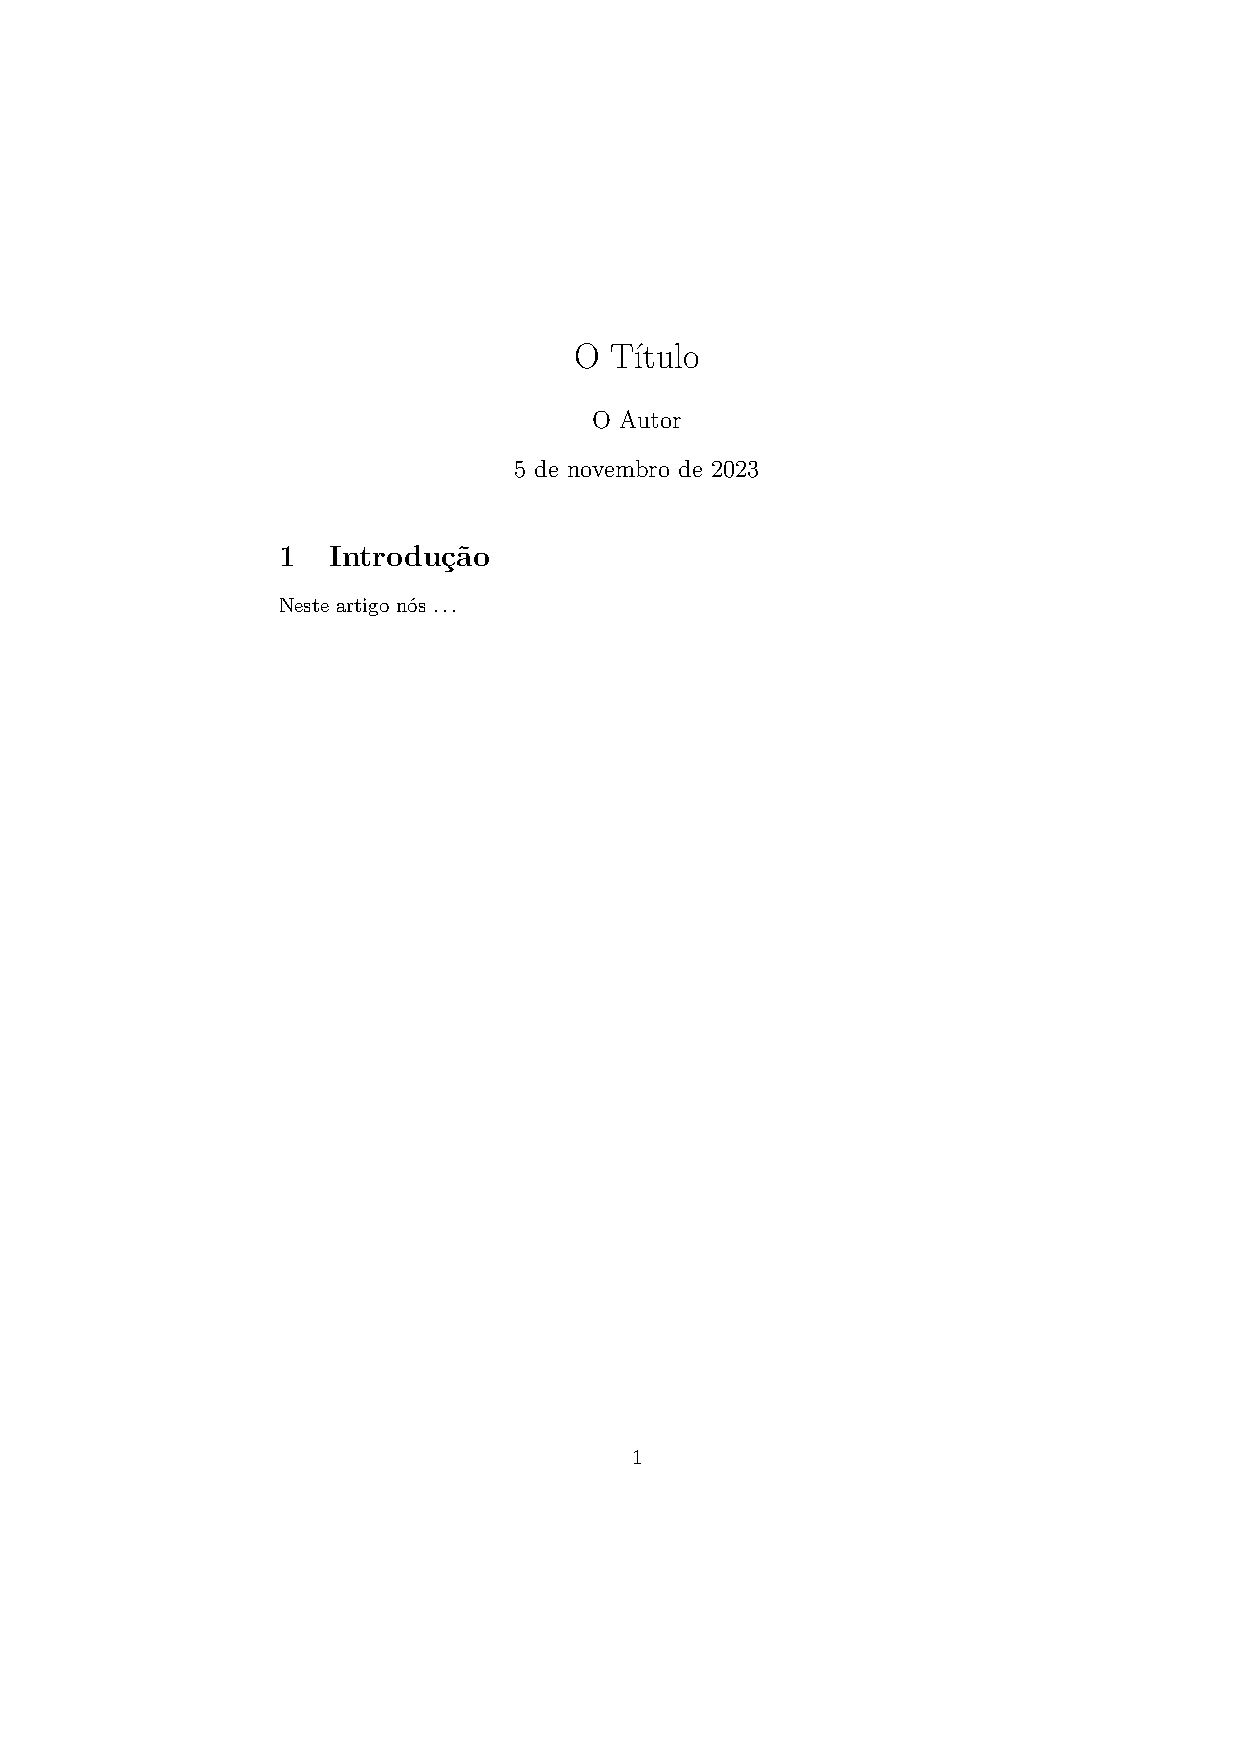
\includegraphics[width=\textwidth,clip,trim=1.5in 7in 3in 2in]{recap-structure.pdf}
\end{minipage}
\end{frame}

%%%%%%%%%%%%%%%%%%%%%%%%%%%%%%%%%%%%%%%%%%%%%%%%%%%%%%%%%%%%%%%%%%%%%%%%%%%%%%%
%%%%%%%%%%%%%%%%%%%%%%%%%%%%%%%%%%%%%%%%%%%%%%%%%%%%%%%%%%%%%%%%%%%%%%%%%%%%%%%
%%%%%%%%%%%%%%%%%%%%%%%%%%%%%%%%%%%%%%%%%%%%%%%%%%%%%%%%%%%%%%%%%%%%%%%%%%%%%%%
\begin{frame}[fragile]{\insertsection: Exercícios}

\begin{enumerate}
\item Aqui você encontra um texto para um pequeno artigo:\footnote{Baseado em \url{http://www.cgd.ucar.edu/cms/agu/scientific_talk.html}}
\begin{center}
\fbox{\href{\wlnewdoc{recap-exercise.tex}}{%
Clique aqui para abrir o exercícios no  \wllogo{}}}
\end{center}
\vskip 2ex
\item Adicione comandos \LaTeX{} ao texto para ficar parecido com este arquivo:
\begin{center}
\fbox{\href{\fileuri/recap-exercise-solution.pdf} de porcentagem, \emph{adicione} a barra invertida (\cmdbs{\%}).
\item Para digitar a equação, use o comando \cmdbs{frac} para fração e  os comandos \cmdbs{left(} and \cmdbs{right)} para os parênteses ficarem com tamanho adequado.
\end{itemize}
\end{block}
\end{frame}

%%%%%%%%%%%%%%%%%%%%%%%%%%%%%%%%%%%%%%%%%%%%%%%%%%%%%%%%%%%%%%%%%%%%%%%%%%%%%%%
%%%%%%%%%%%%%%%%%%%%%%%%%%%%%%%%%%%%%%%%%%%%%%%%%%%%%%%%%%%%%%%%%%%%%%%%%%%%%%%
%%%%%%%%%%%%%%%%%%%%%%%%%%%%%%%%%%%%%%%%%%%%%%%%%%%%%%%%%%%%%%%%%%%%%%%%%%%%%%%
\section{Apresentações com \protect\bftt{beamer}}

%%%%%%%%%%%%%%%%%%%%%%%%%%%%%%%%%%%%%%%%%%%%%%%%%%%%%%%%%%%%%%%%%%%%%%%%%%%%%%%
%%%%%%%%%%%%%%%%%%%%%%%%%%%%%%%%%%%%%%%%%%%%%%%%%%%%%%%%%%%%%%%%%%%%%%%%%%%%%%%
%%%%%%%%%%%%%%%%%%%%%%%%%%%%%%%%%%%%%%%%%%%%%%%%%%%%%%%%%%%%%%%%%%%%%%%%%%%%%%%
\begin{frame}[fragile]{\insertsection}
\begin{itemize}
\item Beamer é um pacote para criar apresentações  (tais como esta!) em
\LaTeX{}.
\item Usa-se a classe de documento \bftt{beamer}.
\item Usa-se o ambiente \bftt{frame} para criar slides.
\end{itemize}
\begin{minipage}{0.55\linewidth}
\inputminted[fontsize=\tiny,frame=single,resetmargins]{latex}%
  {beamer-minimal.tex}
\end{minipage}
\begin{minipage}{0.35\linewidth}
% trim: l b r t
\includegraphics[width=\textwidth,clip,trim=1in 1in 1in 1in]{beamer-minimal.pdf}
\end{minipage}
\end{frame}

%%%%%%%%%%%%%%%%%%%%%%%%%%%%%%%%%%%%%%%%%%%%%%%%%%%%%%%%%%%%%%%%%%%%%%%%%%%%%%%
%%%%%%%%%%%%%%%%%%%%%%%%%%%%%%%%%%%%%%%%%%%%%%%%%%%%%%%%%%%%%%%%%%%%%%%%%%%%%%%
%%%%%%%%%%%%%%%%%%%%%%%%%%%%%%%%%%%%%%%%%%%%%%%%%%%%%%%%%%%%%%%%%%%%%%%%%%%%%%%
\begin{frame}[fragile]{\insertsection: Continuando}

\begin{itemize}
\item A partir de agora, ao passarmos aos próximos slides, tente os exemplos digitando-os no modelo que se encontra no \wllogo.
\end{itemize}
\vskip 2ex
\begin{center}
\fbox{\href{\wlnewdoc{beamer-minimal.tex}}{%
Clique aqui para abrir o modelo no \wllogo{}}}
\end{center}
\end{frame}

%%%%%%%%%%%%%%%%%%%%%%%%%%%%%%%%%%%%%%%%%%%%%%%%%%%%%%%%%%%%%%%%%%%%%%%%%%%%%%%
%%%%%%%%%%%%%%%%%%%%%%%%%%%%%%%%%%%%%%%%%%%%%%%%%%%%%%%%%%%%%%%%%%%%%%%%%%%%%%%
%%%%%%%%%%%%%%%%%%%%%%%%%%%%%%%%%%%%%%%%%%%%%%%%%%%%%%%%%%%%%%%%%%%%%%%%%%%%%%%
\begin{frame}[fragile]
\frametitle{\insertsection: \emph{Slides}}
\begin{itemize}
\item Use o comando \cmdbs{frametitle} para colocar título nos slides.
\item Adicione então conteúdo aos slides.
\item A fonte para esse slide parece-se com isso:
\vskip 2ex
\inputminted[fontsize=\scriptsize,frame=single,resetmargins]{latex}%
  {beamer-frame.tex}
\end{itemize}
\end{frame}

%%%%%%%%%%%%%%%%%%%%%%%%%%%%%%%%%%%%%%%%%%%%%%%%%%%%%%%%%%%%%%%%%%%%%%%%%%%%%%%
%%%%%%%%%%%%%%%%%%%%%%%%%%%%%%%%%%%%%%%%%%%%%%%%%%%%%%%%%%%%%%%%%%%%%%%%%%%%%%%
%%%%%%%%%%%%%%%%%%%%%%%%%%%%%%%%%%%%%%%%%%%%%%%%%%%%%%%%%%%%%%%%%%%%%%%%%%%%%%%
\begin{frame}[fragile]{\insertsection: Seções}
\begin{itemize}
\item  Use o comando \cmdbs{section} para agrupar seus \bftt{slides}s, e o
\bftt{beamer} irá usá-los para criar um sumário automaticamente.
\item Para gerar o sumário, use o comando \cmdbs{tableofcontents}. Aqui está o desta apresentação.
A opção \bftt{currentsection}  destaca a seção atual.
\vskip 2ex
\begin{exampletwouptiny}
\tableofcontents[currentsection]
\end{exampletwouptiny}
\end{itemize}
\end{frame}

%%%%%%%%%%%%%%%%%%%%%%%%%%%%%%%%%%%%%%%%%%%%%%%%%%%%%%%%%%%%%%%%%%%%%%%%%%%%%%%
%%%%%%%%%%%%%%%%%%%%%%%%%%%%%%%%%%%%%%%%%%%%%%%%%%%%%%%%%%%%%%%%%%%%%%%%%%%%%%%
%%%%%%%%%%%%%%%%%%%%%%%%%%%%%%%%%%%%%%%%%%%%%%%%%%%%%%%%%%%%%%%%%%%%%%%%%%%%%%%
\begin{frame}[fragile]{\insertsection: Múltiplas Colunas}
\begin{columns}
\begin{column}{0.4\textwidth}
\begin{itemize}
\item Use os ambientes \bftt{columns} e \bftt{column} para quebrar o slide em colunas.
\item O argumento para cada  \bftt{column} determina sua largura.
\item Veja também o pacote \bftt{multicol}, que quebra automaticamente  seu conteúdo em colunas.
\end{itemize}
\end{column}
\begin{column}{0.6\textwidth}
\begin{minted}[fontsize=\scriptsize,frame=single]{latex}
\begin{columns}
  \begin{column}{0.4\textwidth}
    \begin{itemize}
    \item Use as colunas \ldots
    \item O argumento \ldots
    \item Veja também \ldots
    \end{itemize}
  \end{column}
  \begin{column}{0.6\textwidth}
    % segunda coluna
  \end{column}
\end{columns}
\end{minted}
\end{column}
\end{columns}
\end{frame}

%%%%%%%%%%%%%%%%%%%%%%%%%%%%%%%%%%%%%%%%%%%%%%%%%%%%%%%%%%%%%%%%%%%%%%%%%%%%%%%
%%%%%%%%%%%%%%%%%%%%%%%%%%%%%%%%%%%%%%%%%%%%%%%%%%%%%%%%%%%%%%%%%%%%%%%%%%%%%%%
%%%%%%%%%%%%%%%%%%%%%%%%%%%%%%%%%%%%%%%%%%%%%%%%%%%%%%%%%%%%%%%%%%%%%%%%%%%%%%%
\begin{frame}[fragile]{\insertsection: Destaques}
\begin{itemize}

\item Use \cmdbs{emph} ou \cmdbs{alert} para destacar:
\vskip 1ex
\begin{exampletwouptiny}
Eu devo \emph{enfatizar} que este é
um ponto \alert{importante}.
\end{exampletwouptiny}
\vskip 1ex

\item Ou especifique se quer negrito ou itálico:
\vskip 1ex
\begin{exampletwouptiny}
Texto em \textbf{negrito}.
Texto em \textit{itálico}.
\end{exampletwouptiny}
\vskip 1ex

\item Ou especifique a cor (em inglês Americano):
\vskip 1ex
\begin{exampletwouptiny}
Aqui \textcolor{red}{para}
e \textcolor{green}{começa}.
\end{exampletwouptiny}
\vskip 1ex
\item Veja \url{https://joerglenhard.wordpress.com/2011/08/01/beamer-customization-colors/}
para mais cores \& cores customizadas.
\end{itemize}
\end{frame}

%%%%%%%%%%%%%%%%%%%%%%%%%%%%%%%%%%%%%%%%%%%%%%%%%%%%%%%%%%%%%%%%%%%%%%%%%%%%%%%
%%%%%%%%%%%%%%%%%%%%%%%%%%%%%%%%%%%%%%%%%%%%%%%%%%%%%%%%%%%%%%%%%%%%%%%%%%%%%%%
%%%%%%%%%%%%%%%%%%%%%%%%%%%%%%%%%%%%%%%%%%%%%%%%%%%%%%%%%%%%%%%%%%%%%%%%%%%%%%%
\begin{frame}[fragile]{\insertsection: Figuras}
\begin{itemize}
\item Usa-se \cmdbs{includegraphics} do pacote \bftt{graphicx}.
\item o ambiente \bftt{figure} centraliza por padrão, no \bftt{beamer}.
\vskip 2ex
\begin{exampletwouptiny}
\begin{figure}

\includegraphics[
  width=0.5\textwidth]{gerbil}
\end{figure}
\end{exampletwouptiny}
\end{itemize}
\end{frame}

%%%%%%%%%%%%%%%%%%%%%%%%%%%%%%%%%%%%%%%%%%%%%%%%%%%%%%%%%%%%%%%%%%%%%%%%%%%%%%%
%%%%%%%%%%%%%%%%%%%%%%%%%%%%%%%%%%%%%%%%%%%%%%%%%%%%%%%%%%%%%%%%%%%%%%%%%%%%%%%
%%%%%%%%%%%%%%%%%%%%%%%%%%%%%%%%%%%%%%%%%%%%%%%%%%%%%%%%%%%%%%%%%%%%%%%%%%%%%%%
\begin{frame}[fragile]{\insertsection: Tabelas}
\begin{itemize}
\item Tabelas em \LaTeX{} precisam de atenção.
\item Use o ambiente \bftt{tabular} do pacote \bftt{tabularx}.
\item Os argumento que especificam o alinhamento das colunas: \textbf{l} para esquerda (\emph{left}), \textbf{c} para centralizar e \textbf{r} para direita (\emph{right}).
\begin{exampletwouptiny}
\begin{tabular}{lcr}
Item    & Qtd. & Unid. \$ \\
Celular & 1    & 399,99  \\
Capa    & 2    & 99,99  \\
Cabo    & 3    & 19,99   \\
\end{tabular}
\end{exampletwouptiny}
\item É necessário especificar as linhas verticais. Para as linhas horizontais,  use o
comando \cmdbs{hline}.
\begin{exampletwouptiny}
\begin{tabular}{|l|c|r|} \hline
Item    & Qtd. & Unid. \$ \\\hline
Celular & 1    & 399,99  \\
Capa    & 2    & 99,99  \\
Cabo    & 3    & 19,99   \\\hline
\end{tabular}
\end{exampletwouptiny}
\item Use o ``E comercial''  \keystrokebftt{\&} para separar colunas e barras
invertidas duplas \keystrokebftt{\bs}\keystrokebftt{\bs} para iniciar uma nova
linha (como no ambiente  \bftt{align*} que vimos na parte 1).
\end{itemize}
\end{frame}

%%%%%%%%%%%%%%%%%%%%%%%%%%%%%%%%%%%%%%%%%%%%%%%%%%%%%%%%%%%%%%%%%%%%%%%%%%%%%%%
%%%%%%%%%%%%%%%%%%%%%%%%%%%%%%%%%%%%%%%%%%%%%%%%%%%%%%%%%%%%%%%%%%%%%%%%%%%%%%%
%%%%%%%%%%%%%%%%%%%%%%%%%%%%%%%%%%%%%%%%%%%%%%%%%%%%%%%%%%%%%%%%%%%%%%%%%%%%%%%
\begin{frame}[fragile]{\insertsection: Blocos}
\begin{itemize}
\item Um ambiente \bftt{block} produz uma caixa com título.
\begin{exampletwouptiny}
\begin{block}{Fato interessante}
Isto é importante.
\end{block}

\begin{alertblock}{Atenção}
Isto é realmente importante!
\end{alertblock}
\end{exampletwouptiny}

\item A aparência dos blocos depende do tema escolhido \ldots
\end{itemize}
\end{frame}

%%%%%%%%%%%%%%%%%%%%%%%%%%%%%%%%%%%%%%%%%%%%%%%%%%%%%%%%%%%%%%%%%%%%%%%%%%%%%%%
%%%%%%%%%%%%%%%%%%%%%%%%%%%%%%%%%%%%%%%%%%%%%%%%%%%%%%%%%%%%%%%%%%%%%%%%%%%%%%%
%%%%%%%%%%%%%%%%%%%%%%%%%%%%%%%%%%%%%%%%%%%%%%%%%%%%%%%%%%%%%%%%%%%%%%%%%%%%%%%
\begin{frame}[fragile]
\frametitle{\insertsection: Temas}
\begin{itemize}
\item Altere a aparência de  suas apresentações  usando \alert{temas}.
\item Veja \url{http://deic.uab.es/~iblanes/beamer_gallery/index_by_theme.html}
para uma grande coleção de temas.
\end{itemize}
\begin{minipage}{0.55\linewidth}
\inputminted[fontsize=\scriptsize,frame=single,resetmargins]{latex}%
  {beamer-theme.tex}
\end{minipage}
\begin{minipage}{0.35\linewidth}
% trim: l b r t
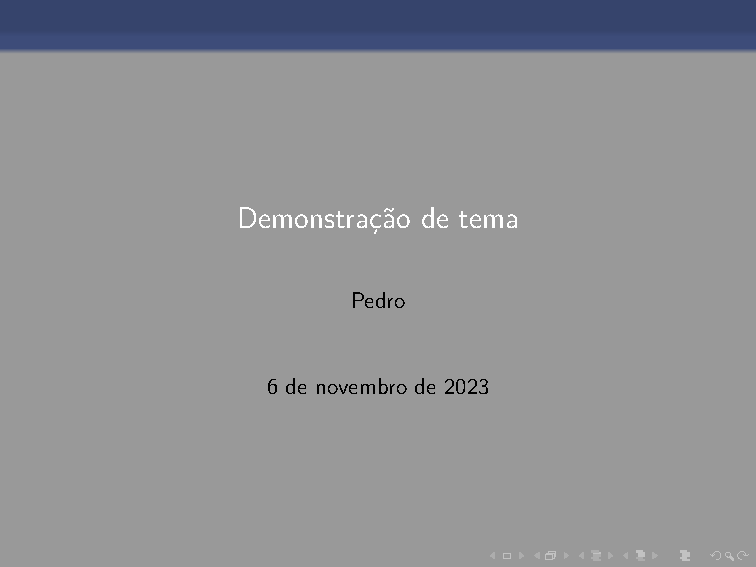
\includegraphics[width=\textwidth]{beamer-theme.pdf}
\end{minipage}
\end{frame}

%%%%%%%%%%%%%%%%%%%%%%%%%%%%%%%%%%%%%%%%%%%%%%%%%%%%%%%%%%%%%%%%%%%%%%%%%%%%%%%
%%%%%%%%%%%%%%%%%%%%%%%%%%%%%%%%%%%%%%%%%%%%%%%%%%%%%%%%%%%%%%%%%%%%%%%%%%%%%%%
%%%%%%%%%%%%%%%%%%%%%%%%%%%%%%%%%%%%%%%%%%%%%%%%%%%%%%%%%%%%%%%%%%%%%%%%%%%%%%%
\begin{frame}[fragile]{\insertsection: Animação}
\begin{itemize}
\item Um \emph{frame} pode gerar múltiplos slides.
\item Usa-se o comando \cmdbs{pause} para mostrar somente parte do slide.
\vskip 2ex
\begin{exampletwouptinynoframe}
\begin{itemize}
\item Você pode sentir a
\pause \item antecipação?
\end{itemize}
\end{exampletwouptinynoframe}
\vskip 2ex
\item Existem outras formas de fazer animações no \bftt{beamer}; veja também
os comandos \cmdbs{only}, \cmdbs{alt}, e \cmdbs{uncover}.
\end{itemize}
\end{frame}

%%%%%%%%%%%%%%%%%%%%%%%%%%%%%%%%%%%%%%%%%%%%%%%%%%%%%%%%%%%%%%%%%%%%%%%%%%%%%%%
%%%%%%%%%%%%%%%%%%%%%%%%%%%%%%%%%%%%%%%%%%%%%%%%%%%%%%%%%%%%%%%%%%%%%%%%%%%%%%%
%%%%%%%%%%%%%%%%%%%%%%%%%%%%%%%%%%%%%%%%%%%%%%%%%%%%%%%%%%%%%%%%%%%%%%%%%%%%%%%
\begin{frame}[fragile]{\insertsection: Exercício}

Recrie a apresentação ``Revolução dos Cravos'' em \bftt{beamer}.

\begin{enumerate}
\item Abra o exercício no \wllogo{}:
\begin{center}
\fbox{\href{\wlnewdoc{beamer-exercise.tex}}{%
Clique para abrir esse exercício no \wllogo{}}}
\end{center}
\vskip 2ex
\item Baixe esta imagem no seu computador e faça o \emph{upload} para o \wllogo{} usando o menu.
\begin{center}
\fbox{\href{\fileuri/Cravos.png?dl=1}{Clique para baixar a imagem}}
\end{center}
\vskip 2ex
\item Adicione comandos \LaTeX{} para seu \bftt{.tex} e faça parecer como esta aqui:
\begin{center}
\fbox{\href{\fileuri/beamer-exercise-solution.pdf}{%
Clique para abrir o modelo do documento}}
\end{center}
\end{enumerate}
\end{frame}

%%%%%%%%%%%%%%%%%%%%%%%%%%%%%%%%%%%%%%%%%%%%%%%%%%%%%%%%%%%%%%%%%%%%%%%%%%%%%%%
%%%%%%%%%%%%%%%%%%%%%%%%%%%%%%%%%%%%%%%%%%%%%%%%%%%%%%%%%%%%%%%%%%%%%%%%%%%%%%%
%%%%%%%%%%%%%%%%%%%%%%%%%%%%%%%%%%%%%%%%%%%%%%%%%%%%%%%%%%%%%%%%%%%%%%%%%%%%%%%
\section{Desenhando com \protect\tikzname}

%%%%%%%%%%%%%%%%%%%%%%%%%%%%%%%%%%%%%%%%%%%%%%%%%%%%%%%%%%%%%%%%%%%%%%%%%%%%%%%
%%%%%%%%%%%%%%%%%%%%%%%%%%%%%%%%%%%%%%%%%%%%%%%%%%%%%%%%%%%%%%%%%%%%%%%%%%%%%%%
%%%%%%%%%%%%%%%%%%%%%%%%%%%%%%%%%%%%%%%%%%%%%%%%%%%%%%%%%%%%%%%%%%%%%%%%%%%%%%%
\begin{frame}[fragile]{\insertsection}
\begin{itemize}
\item \tikzname{} é um pacote para desenhar figuras em \LaTeX.
\item Define uma poderosa linguagem de desenho dentro do  \LaTeX{}. Códigos curtos podem desenhar coisas surpreendentemente complicadas.
\begin{figure}
\href{http://www.texample.net/tikz/examples/rotated-triangle/}{%
  \includegraphics[width=0.35\textwidth]{rotated-triangle}}
\end{figure}
\item Começaremos com coisas simples. Para desenhar um segmento de reta  em \tikzname:
\vskip 1ex
\begin{exampletwouptiny}
\begin{tikzpicture}
\draw (0,0) -- (1,1); % um segmetno de  reta
\end{tikzpicture}
\end{exampletwouptiny}
\end{itemize}
\end{frame}

%%%%%%%%%%%%%%%%%%%%%%%%%%%%%%%%%%%%%%%%%%%%%%%%%%%%%%%%%%%%%%%%%%%%%%%%%%%%%%%
%%%%%%%%%%%%%%%%%%%%%%%%%%%%%%%%%%%%%%%%%%%%%%%%%%%%%%%%%%%%%%%%%%%%%%%%%%%%%%%
%%%%%%%%%%%%%%%%%%%%%%%%%%%%%%%%%%%%%%%%%%%%%%%%%%%%%%%%%%%%%%%%%%%%%%%%%%%%%%%
\begin{frame}[fragile]{\insertsection: Coordenadas}
\begin{itemize}
\item O padrão para coordenadas são em centímetros, com o sentido usual:
\begin{figure}
\begin{tikzpicture}[scale=0.5]
\draw[help lines] (0,0) grid (3,3);
\node[below left] at (0,0) {$(0,0)$};
\node[below right] at (3,0) {$(3,0)$};
\node[above right] at (3,3) {$(3,3)$};
\node[above left] at (0,3) {$(0,3)$};
\end{tikzpicture}
\end{figure}
\item Quando você está trabalhando com \tikzname, linhas de grade são de grande ajuda:
\vskip 1ex
\begin{exampletwouptiny}
\begin{tikzpicture}
\draw[help lines] (0,0) grid (3,3);
\end{tikzpicture}
\end{exampletwouptiny}
\end{itemize}
\end{frame}

%%%%%%%%%%%%%%%%%%%%%%%%%%%%%%%%%%%%%%%%%%%%%%%%%%%%%%%%%%%%%%%%%%%%%%%%%%%%%%%
%%%%%%%%%%%%%%%%%%%%%%%%%%%%%%%%%%%%%%%%%%%%%%%%%%%%%%%%%%%%%%%%%%%%%%%%%%%%%%%
%%%%%%%%%%%%%%%%%%%%%%%%%%%%%%%%%%%%%%%%%%%%%%%%%%%%%%%%%%%%%%%%%%%%%%%%%%%%%%%
\begin{frame}[fragile]{\insertsection: Lines}
\begin{itemize}
\item Tipos de flecha e estilo de linhas são especificadas como opções ao comando \cmdbs{draw}.
\item Cada comando de desenho deve ser finalizado com um ponto e vírgula: \keystrokebftt{;}.
\vskip 1ex
\begin{exampletwouptiny}
\begin{tikzpicture}
\draw[help lines] (0,0) grid (3,3);
\draw[->] (0,0) -- (1,1);
\draw[<->, thick] (2,1) -- (1,2);
\draw[<-, thick, dashed] (2,2)--(3,3);
\end{tikzpicture}
\end{exampletwouptiny}
\end{itemize}
\end{frame}

%%%%%%%%%%%%%%%%%%%%%%%%%%%%%%%%%%%%%%%%%%%%%%%%%%%%%%%%%%%%%%%%%%%%%%%%%%%%%%%
%%%%%%%%%%%%%%%%%%%%%%%%%%%%%%%%%%%%%%%%%%%%%%%%%%%%%%%%%%%%%%%%%%%%%%%%%%%%%%%
%%%%%%%%%%%%%%%%%%%%%%%%%%%%%%%%%%%%%%%%%%%%%%%%%%%%%%%%%%%%%%%%%%%%%%%%%%%%%%%
\begin{frame}[fragile]{\insertsection: Caminhos}
\begin{itemize}
\item Você pode especificar múltiplos pontos para formar um caminho.
\item Flechas aparecerão apenas no final do caminho.
\vskip 1ex
\begin{exampletwouptiny}
\begin{tikzpicture}
\draw[help lines] (0,0) grid (3,3);
% axes:
\draw[<->, thick] (0,3)--(0,0)--(3,0);
% diamond:
\draw (1.5,0.5) -- (2.5,1.5) --
      (1.5,2.5) -- (0.5,1.5) --
      cycle; % close the path
\end{tikzpicture}
\end{exampletwouptiny}
\end{itemize}
\end{frame}

%%%%%%%%%%%%%%%%%%%%%%%%%%%%%%%%%%%%%%%%%%%%%%%%%%%%%%%%%%%%%%%%%%%%%%%%%%%%%%%
%%%%%%%%%%%%%%%%%%%%%%%%%%%%%%%%%%%%%%%%%%%%%%%%%%%%%%%%%%%%%%%%%%%%%%%%%%%%%%%
%%%%%%%%%%%%%%%%%%%%%%%%%%%%%%%%%%%%%%%%%%%%%%%%%%%%%%%%%%%%%%%%%%%%%%%%%%%%%%%
\begin{frame}[fragile]{\insertsection: Cores}
\begin{itemize}
\item Cores são também especificadas como opções ao comanado \cmdbs{draw}.
\vskip 1ex
\begin{exampletwouptiny}
\begin{tikzpicture}
\draw[help lines] (0,0) grid (3,3);
% axes
\draw[<->, thick, red]
  (0,3)--(0,0)--(3,0);
% diamond
\draw[thick, blue, fill=yellow]
  (1.5,0.5) -- (2.5,1.5) --
  (1.5,2.5) -- (0.5,1.5) --
  cycle;
\end{tikzpicture}
\end{exampletwouptiny}
\end{itemize}
\end{frame}

%%%%%%%%%%%%%%%%%%%%%%%%%%%%%%%%%%%%%%%%%%%%%%%%%%%%%%%%%%%%%%%%%%%%%%%%%%%%%%%
%%%%%%%%%%%%%%%%%%%%%%%%%%%%%%%%%%%%%%%%%%%%%%%%%%%%%%%%%%%%%%%%%%%%%%%%%%%%%%%
%%%%%%%%%%%%%%%%%%%%%%%%%%%%%%%%%%%%%%%%%%%%%%%%%%%%%%%%%%%%%%%%%%%%%%%%%%%%%%%
\begin{frame}[fragile]{\insertsection: Formas}
\begin{itemize}
\item \tikzname{} tem comandos internos para formas simples.
\vskip 1ex
\begin{exampletwouptiny}
\begin{tikzpicture}
\draw[help lines] (0,0) grid (3,3);
\draw (1.5,2.0) circle (0.5);
\draw (0.5,0.5) rectangle (2.5,1.5);
\end{tikzpicture}
\end{exampletwouptiny}
\end{itemize}
\end{frame}

%%%%%%%%%%%%%%%%%%%%%%%%%%%%%%%%%%%%%%%%%%%%%%%%%%%%%%%%%%%%%%%%%%%%%%%%%%%%%%%
%%%%%%%%%%%%%%%%%%%%%%%%%%%%%%%%%%%%%%%%%%%%%%%%%%%%%%%%%%%%%%%%%%%%%%%%%%%%%%%
%%%%%%%%%%%%%%%%%%%%%%%%%%%%%%%%%%%%%%%%%%%%%%%%%%%%%%%%%%%%%%%%%%%%%%%%%%%%%%%
\begin{frame}[fragile]{\insertsection: Nós \& Legendas}
\begin{itemize}
\item Utilize nós (comando \cmdbs{node}) para colocar texto (e texto matemático) em desenhos do \tikzname{}.
\item Você também pode utilizar nós como coordenadas --- muito útil para diagramas.
\vskip 1ex
\begin{exampletwouptiny}
\begin{tikzpicture}
\draw[help lines] (0,0) grid (3,3);
\node (h) at (0,0) {H};
\node (x) at (1.5,1.5) {$\xi$};
\node (t) at (3,0) {T};
\draw[->] (x) -- (h);
\draw[->] (x) -- (t);
\end{tikzpicture}
\end{exampletwouptiny}
\end{itemize}
\end{frame}

%%%%%%%%%%%%%%%%%%%%%%%%%%%%%%%%%%%%%%%%%%%%%%%%%%%%%%%%%%%%%%%%%%%%%%%%%%%%%%%
%%%%%%%%%%%%%%%%%%%%%%%%%%%%%%%%%%%%%%%%%%%%%%%%%%%%%%%%%%%%%%%%%%%%%%%%%%%%%%%
%%%%%%%%%%%%%%%%%%%%%%%%%%%%%%%%%%%%%%%%%%%%%%%%%%%%%%%%%%%%%%%%%%%%%%%%%%%%%%%
\begin{frame}[fragile]{\insertsection: Funções}
\begin{itemize}
\item Também é possível graficar algumas funções simples.
\vskip 1ex
\begin{exampletwouptiny}
\begin{tikzpicture}[scale=0.5]
% y axis
\draw[<->, thick] (0,2) -- (0,-2);
% x axis
\draw[ ->, thick] (0,0) -- (7, 0);
% curves
\draw[cyan,domain=0:2*pi]
  plot (\x, {sin(\x r)});
\draw[magenta,domain=0:2*pi]
  plot (\x, {cos(\x r)});
\end{tikzpicture}
\end{exampletwouptiny}
\end{itemize}
\end{frame}

%%%%%%%%%%%%%%%%%%%%%%%%%%%%%%%%%%%%%%%%%%%%%%%%%%%%%%%%%%%%%%%%%%%%%%%%%%%%%%%
%%%%%%%%%%%%%%%%%%%%%%%%%%%%%%%%%%%%%%%%%%%%%%%%%%%%%%%%%%%%%%%%%%%%%%%%%%%%%%%
%%%%%%%%%%%%%%%%%%%%%%%%%%%%%%%%%%%%%%%%%%%%%%%%%%%%%%%%%%%%%%%%%%%%%%%%%%%%%%%
\begin{frame}[fragile]{\insertsection: Exemplos}
\begin{itemize}
\item Dê uma olhada em  \fbox{\href{http://texample.net/tikz/}{\TeX{}ample.net}} para muitos outros exemplos com \tikzname{}:
\end{itemize}
\begin{figure}
\href{http://texample.net/tikz/examples/escher-brick-penrose-triangle/}{%
  \includegraphics[width=0.3\textwidth]{escher-brick-penrose-triangle}}
\href{http://texample.net/tikz/examples/computer-science-mindmap/}{%
  \includegraphics[width=0.3\textwidth]{computer-science-mindmap}}
\href{http://texample.net/tikz/examples/gajski-kuhn-y-chart/}{%
  \includegraphics[width=0.3\textwidth]{gajski-kuhn-y-chart}}
\end{figure}
\end{frame}

%%%%%%%%%%%%%%%%%%%%%%%%%%%%%%%%%%%%%%%%%%%%%%%%%%%%%%%%%%%%%%%%%%%%%%%%%%%%%%%
%%%%%%%%%%%%%%%%%%%%%%%%%%%%%%%%%%%%%%%%%%%%%%%%%%%%%%%%%%%%%%%%%%%%%%%%%%%%%%%
%%%%%%%%%%%%%%%%%%%%%%%%%%%%%%%%%%%%%%%%%%%%%%%%%%%%%%%%%%%%%%%%%%%%%%%%%%%%%%%
\begin{frame}[fragile]{\insertsection: Exercício}
Desenhe a figura abaixo em \tikzname:\footnote{Baseado em \url{http://xkcd.com/1022}}
\begin{figure}
\begin{tikzpicture}
\draw[help lines] (0,0) grid (6,6);
\draw[thick] (2,3) circle (0.5);
\draw[thick] (2,2.5) -- (2,1);              % corpo
\draw[thick] (1,1.5) -- (2,2) -- (3,1.5);   % braços
\draw[thick] (1.5, 0) -- (2,1) -- (2.5, 0); % pernas
\draw[blue] (2,4) rectangle (6,6);
\draw[blue] (2.5,3.5) circle (0.1);
\draw[blue] (2.8,3.8) circle (0.15);
\node at (4,5) {E tudo acabou assim.};
\end{tikzpicture}

\end{figure}
\end{frame}

%%%%%%%%%%%%%%%%%%%%%%%%%%%%%%%%%%%%%%%%%%%%%%%%%%%%%%%%%%%%%%%%%%%%%%%%%%%%%%%
%%%%%%%%%%%%%%%%%%%%%%%%%%%%%%%%%%%%%%%%%%%%%%%%%%%%%%%%%%%%%%%%%%%%%%%%%%%%%%%
%%%%%%%%%%%%%%%%%%%%%%%%%%%%%%%%%%%%%%%%%%%%%%%%%%%%%%%%%%%%%%%%%%%%%%%%%%%%%%%
\section{Notas com  \protect\bftt{todonotes}}

%%%%%%%%%%%%%%%%%%%%%%%%%%%%%%%%%%%%%%%%%%%%%%%%%%%%%%%%%%%%%%%%%%%%%%%%%%%%%%%
%%%%%%%%%%%%%%%%%%%%%%%%%%%%%%%%%%%%%%%%%%%%%%%%%%%%%%%%%%%%%%%%%%%%%%%%%%%%%%%
%%%%%%%%%%%%%%%%%%%%%%%%%%%%%%%%%%%%%%%%%%%%%%%%%%%%%%%%%%%%%%%%%%%%%%%%%%%%%%%
\begin{frame}[fragile]{\insertsection}
\begin{itemize}
\item O comando \cmdbs{todo} do pacote \bftt{todonotes} é ótimo para deixar notas em
textos \LaTeX{} para você ou para seus colaboradores.
\begin{exampletwouptiny}
\todo{adicione resultados}
\todo[color=blue!20]{arrume o método}
\end{exampletwouptiny}
\vskip 2ex
\item Dica quente: defina o seu próprio comando com \cmdbs{newcommand}
\begin{minted}[fontsize=\scriptsize,frame=single]{latex}
\newcommand{\alice}[1]{\todo[color=green!40]{#1}}
\newcommand{\bob}[1]{\todo[color=purple!40]{#1}}
\end{minted}
Isso pode economizar muita digitação:
\begin{exampletwouptiny}
\alice{adicione resultados}
\bob{arrume o método}
\end{exampletwouptiny}
\end{itemize}
\end{frame}

%%%%%%%%%%%%%%%%%%%%%%%%%%%%%%%%%%%%%%%%%%%%%%%%%%%%%%%%%%%%%%%%%%%%%%%%%%%%%%%
%%%%%%%%%%%%%%%%%%%%%%%%%%%%%%%%%%%%%%%%%%%%%%%%%%%%%%%%%%%%%%%%%%%%%%%%%%%%%%%
%%%%%%%%%%%%%%%%%%%%%%%%%%%%%%%%%%%%%%%%%%%%%%%%%%%%%%%%%%%%%%%%%%%%%%%%%%%%%%%
\begin{frame}[fragile]{\insertsection}
\begin{columns}
  \begin{column}{0.4\textwidth}
    \begin{itemize}
    \item Apenas notas  \emph{inline} são suportadas pelo \keystrokebftt{beamer}, mas notas na margem são suportadas por documentos normais.
    \item Há também um comando \cmdbs{listoftodos} bem útil.
    \end{itemize}
  \end{column}
  \begin{column}{0.6\textwidth}
    \includegraphics[width=\textwidth,page=1]{todonotes-example}
  \end{column}
\end{columns}
\end{frame}

%%%%%%%%%%%%%%%%%%%%%%%%%%%%%%%%%%%%%%%%%%%%%%%%%%%%%%%%%%%%%%%%%%%%%%%%%%%%%%%
%%%%%%%%%%%%%%%%%%%%%%%%%%%%%%%%%%%%%%%%%%%%%%%%%%%%%%%%%%%%%%%%%%%%%%%%%%%%%%%
%%%%%%%%%%%%%%%%%%%%%%%%%%%%%%%%%%%%%%%%%%%%%%%%%%%%%%%%%%%%%%%%%%%%%%%%%%%%%%%
\section{Planilhas com \protect\bftt{spreadtab}}

%%%%%%%%%%%%%%%%%%%%%%%%%%%%%%%%%%%%%%%%%%%%%%%%%%%%%%%%%%%%%%%%%%%%%%%%%%%%%%%
%%%%%%%%%%%%%%%%%%%%%%%%%%%%%%%%%%%%%%%%%%%%%%%%%%%%%%%%%%%%%%%%%%%%%%%%%%%%%%%
%%%%%%%%%%%%%%%%%%%%%%%%%%%%%%%%%%%%%%%%%%%%%%%%%%%%%%%%%%%%%%%%%%%%%%%%%%%%%%%
\begin{frame}[fragile]{\insertsection}
\begin{itemize}
\item Agora que você viu como \LaTeX{} pode substituir  Word e PowerPoint, que tal Excel?
\item Tarefa: tente o pacote \fbox{\href{http://www.ctan.org/pkg/spreadtab}{\bftt{spreadtab}}}!
\end{itemize}
\end{frame}

%%%%%%%%%%%%%%%%%%%%%%%%%%%%%%%%%%%%%%%%%%%%%%%%%%%%%%%%%%%%%%%%%%%%%%%%%%%%%%%
%%%%%%%%%%%%%%%%%%%%%%%%%%%%%%%%%%%%%%%%%%%%%%%%%%%%%%%%%%%%%%%%%%%%%%%%%%%%%%%
%%%%%%%%%%%%%%%%%%%%%%%%%%%%%%%%%%%%%%%%%%%%%%%%%%%%%%%%%%%%%%%%%%%%%%%%%%%%%%%
\begin{frame}
\begin{center}
Obrigado, e seja feliz escrevendo seus próximos \TeX{}tos!
\end{center}
\end{frame}

\end{document}